

%=========================================================================
% Start of the introduction to work energy integrals
%=========================================================================
\preClass{Vector Components}

\begin{problem}
\item A 2,000 N force is applied to a 500 kg block of sandstone.

  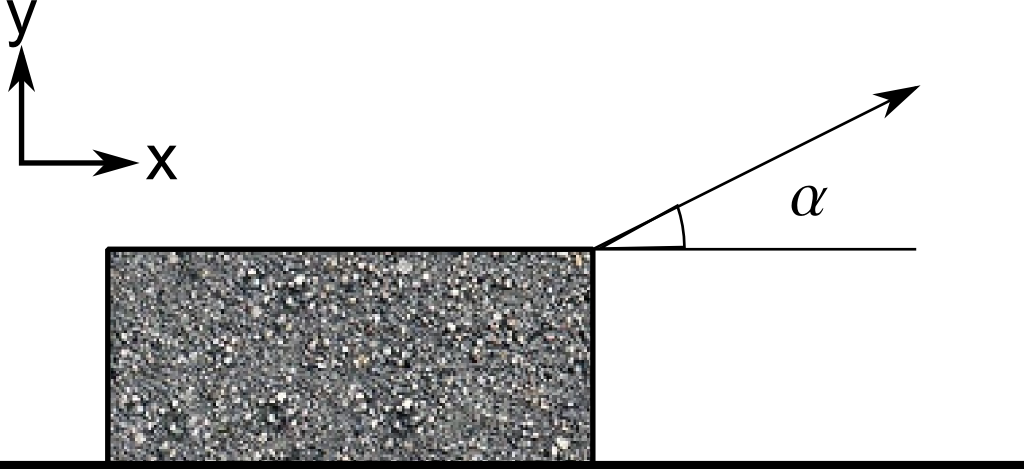
\includegraphics[width=10cm]{ink/week7/dragBlock}

  \begin{subproblem}
  \item If the angle, $\alpha$, is $\frac{\pi}{6}$ determine the
    $\vec{i}$ and $\vec{j}$ components of the force.
    \vfill
  \item If the angle, $\alpha$, is $\frac{\pi}{3}$ determine the
    $\vec{i}$ and $\vec{j}$ components of the force.
    \vfill
  \item If the angle, $\alpha$, is $\frac{2\pi}{3}$ determine the
    $\vec{i}$ and $\vec{j}$ components of the force.
    \vfill
  \end{subproblem}
\end{problem}


\actTitle{Non-Constant Forces}
\begin{problem}
\item A 1,800 N force is applied to a 500 kg block of sandstone. The
  coefficient of friction is 0.2.

  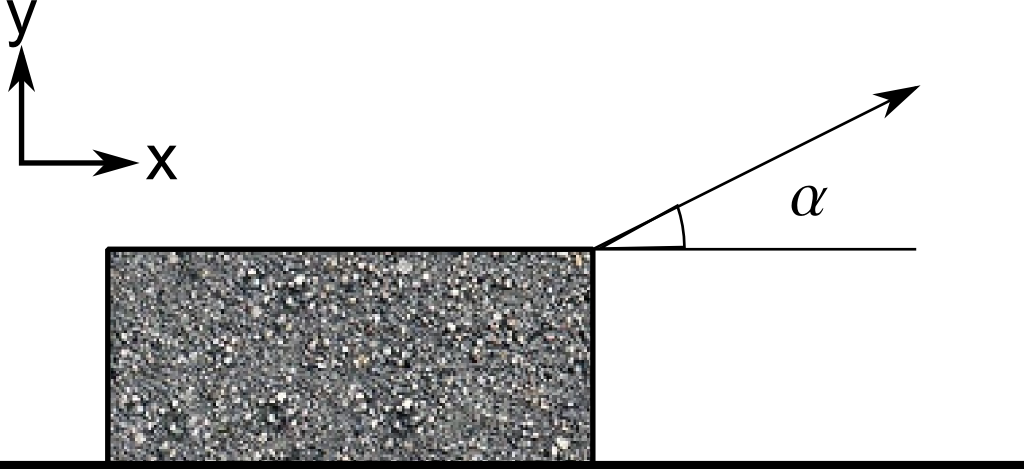
\includegraphics[width=8cm]{ink/week7/dragBlock}

  \begin{subproblem}
    \item Make a sketch of the free body diagram.
      \vspace{6em}
    \item Determine the work done if the block is dragged 10 m and the
      angle is $\alpha=\frac{\pi}{6}$.
      \vfill
    \item Determine the work done if the block is pulled for 20
      seconds and the angle is $\alpha=\frac{\pi}{3}$.  
      \vfill

    \item Determine the smallest angle which can be used and move the
      block.
      \vfill
  \end{subproblem}

  \clearpage

\item Suppose that as the block is pulled the sandstone grinds off on
  the bottom. It starts at a mass of 500 kg. For each meter is moves
  2\% of the sandstone is removed. Assume that the block starts at the
  origin, $x=0$ and assume that the angle is
  $\alpha=\frac{\pi}{6}$. The coefficient of friction is 0.2.

  \begin{subproblem}
  \item Determine the mass of the block given its position.
    \vfill
  \item Determine the amount of force necessary to move the block at a
    constant speed given the block's position.
    \vfill
  \item Make a sketch of the force as a function of the block's
    position.
    \sideNote{ Be sure to label your axes and label all important
      points on your graph.}

    \vfill
  \end{subproblem}

\end{problem}

\actTitle{Work and Riemann Sums}
\begin{problem}
\item The block used in the previous activity is examined, and we wish
  to find the amount of work necessary to pull the block at a constant
  speed over a distance of 100m.  Suppose that as the block is pulled
  the sandstone grinds off on the bottom. It starts at a mass of 500
  kg and is pulled at a constant velocity. For each meter is moves 2\%
  of the sandstone is removed. Assume that the block starts at the
  origin, $x=0$ and assume that the angle is
  $\alpha=\frac{\pi}{6}$. The coefficient of friction is 0.2.

  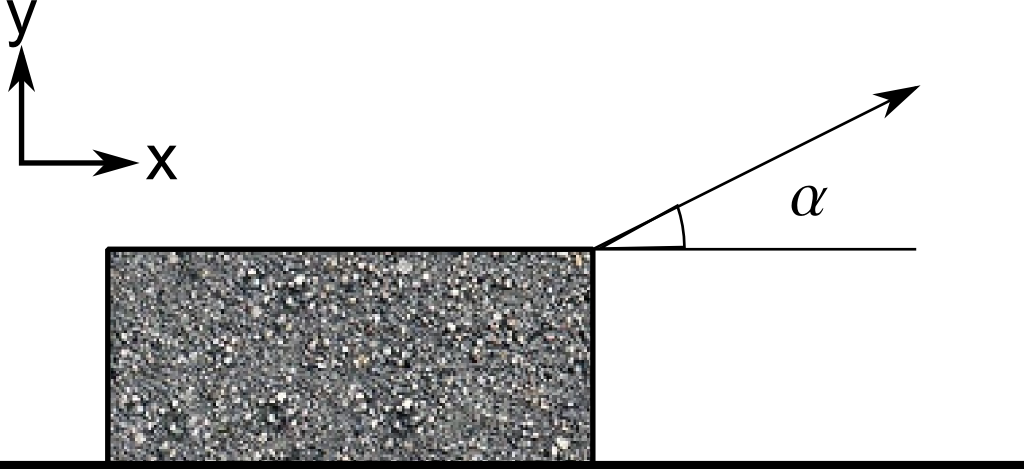
\includegraphics[width=8cm]{ink/week7/dragBlock}

  \begin{subproblem}
  \item Redraw the sketch of the force as a function of the block's
    position.
    \sideNote{ Be sure to label your axes and label all important
      points on your graph.}

    \vfill

  \item Break the distance in five equal lengths across the 100m.  If
    you assume that the force is constant over each interval how much
    work is required to move the block 100m?
    \sideNote{Use the force required at the start of each interval.}

    \vfill

    \clearpage

  \item Break the distance in ten equal lengths across the 100m.  If
    you assume that the force is constant over each interval how much
    work is required to move the block 100m?
    \sideNote{Use the force required at the start of each interval.}

    \vfill

  \item Break the distance in twenty equal lengths across the 100m.  If
    you assume that the force is constant over each interval how much
    work is required to move the block 100m?
    \sideNote{Use the force required at the start of each interval.}

    \vfill

  \item Briefly explain what is happening with respect to your
    approximation of the work. Is it getting bigger or smaller? What
    can you do to make the approximation better?

    \vspace{3em}

  \end{subproblem}
\end{problem}

\postClass

\begin{problem}
\item Briefly state two ideas from today's class.
  \begin{itemize}
  \item 
  \item 
  \end{itemize}
\item 
  \begin{subproblem}
    \item
  \end{subproblem}
\end{problem}


%===============================================================================
% Start of activity on more formal overview of Riemann sums and work integrals.
%===============================================================================
\preClass{Approximation of Work Integrals}

\begin{problem}
\item An arrow is placed in a bow, and the bow is pulled back. The
  force due to the bow string on the arrow is 700N/m multiplied by the
  displacement. 
  \begin{subproblem}
  \item Make a sketch of the force as a function of the displacement.
    \vfill
  \item The maximum force a person can apply to the bow string is
    300N. What is the maximum displacement?
    \vfill
  \item The maximum force a person can apply to the bow string is
    200N. What is the maximum displacement?
    \vfill
  \end{subproblem}
\end{problem}


\actTitle{Approximation of Work Integrals}
\begin{problem}
\item An arrow is placed in a bow, and the bow is pulled back. The
  force due to the bow string on the arrow is 70N/m multiplied by the
  displacement. 
  \begin{subproblem}
  \item Make a sketch of the free body diagram of the arrow.
    \sideNote{label the angle between the force applied to the arrow
      and the direction of movement of the arrow.}  
    \vfill
  \item The maximum force a person can apply to the bow string is
    250N. What is the maximum displacement?  
    \vfill
  \item Make a sketch of the force as a function of the displacement
    from 0m to the maximum displacement.
    \vfill
    \clearpage
  \item Make an approximation of the work performed on the arrow over
    the first 0.05m when it is released.
    \vfill
  \item If the movement is divided up into 100 equally spaced segments
    determine the force at the start of any segment.
    \vfill
  \item Use the formula for the force to construct an approximation
    for the total work performed on the arrow if it is released from
    the maximum distance.
    \vfill
  \end{subproblem}
\end{problem}

\actTitle{The Riemann Sum}
\begin{problem}
\item An arrow is placed in a bow, and the bow is pulled back. The
  force due to the bow string on the arrow is 70N/m multiplied by the
  displacement. 
  \begin{subproblem}
  \item Make a sketch of the free body diagram of the arrow.
    \sideNote{label the angle between the force applied to the arrow
      and the direction of movement of the arrow.}  \vfill
  \item The maximum force a person can apply to the bow string is
    250N. What is the maximum displacement?  
    \vfill
  \item Make a sketch of the force as a function of the displacement
    from 0m to the maximum displacement.
    \vfill
    \clearpage
  \item If the movement is divided up into $N$ equally spaced segments
    determine the force at the start of any segment.
    \vfill
  \item Determine the total work performed over any one segment.
    \vfill
  \item Use the formula for the force to construct an approximation
    for the total work performed on the arrow if it is released from
    the maximum distance.
    \vfill
  \item What can you do to refine and make a more accurate estimate of
    the work?
  \end{subproblem}
\end{problem}

\postClass

\begin{problem}
\item Briefly state two ideas from today's class.
  \begin{itemize}
  \item 
  \item 
  \end{itemize}
\item 
  \begin{subproblem}
    \item
  \end{subproblem}
\end{problem}




%%% Local Variables:
%%% mode: latex
%%% TeX-master: "labManual"
%%% End:

